\documentclass[portrait,final,a0paper]{baposter}
%\documentclass[a4shrink,portrait,final]{baposter}
% Usa a4shrink for an a4 sized paper.

\tracingstats=2

\usepackage{calc}
\usepackage{graphicx}
\usepackage{amsmath}
\usepackage{amssymb}
\usepackage{relsize}
\usepackage{multirow}
\usepackage{bm}

\usepackage{graphicx}
\usepackage{multicol}

\usepackage{pgfbaselayers}
\pgfdeclarelayer{background}
\pgfdeclarelayer{foreground}
\pgfsetlayers{background,main,foreground}

\usepackage{times}
\usepackage{helvet}
%\usepackage{bookman}
\usepackage{palatino}

\newcommand{\captionfont}{\footnotesize}

\selectcolormodel{cmyk}

\graphicspath{{images/}}

%%%%%%%%%%%%%%%%%%%%%%%%%%%%%%%%%%%%%%%%%%%%%%%%%%%%%%%%%%%%%%%%%%%%%%%%%%%%%%%%
%%%% Some math symbols used in the text
%%%%%%%%%%%%%%%%%%%%%%%%%%%%%%%%%%%%%%%%%%%%%%%%%%%%%%%%%%%%%%%%%%%%%%%%%%%%%%%%
% Format 
\newcommand{\Matrix}[1]{\begin{bmatrix} #1 \end{bmatrix}}
\newcommand{\Vector}[1]{\Matrix{#1}}
\newcommand*{\SET}[1]  {\ensuremath{\mathcal{#1}}}
\newcommand*{\MAT}[1]  {\ensuremath{\mathbf{#1}}}
\newcommand*{\VEC}[1]  {\ensuremath{\bm{#1}}}
\newcommand*{\CONST}[1]{\ensuremath{\mathit{#1}}}
\newcommand*{\norm}[1]{\mathopen\| #1 \mathclose\|}% use instead of $\|x\|$
\newcommand*{\abs}[1]{\mathopen| #1 \mathclose|}% use instead of $\|x\|$
\newcommand*{\absLR}[1]{\left| #1 \right|}% use instead of $\|x\|$

\def\norm#1{\mathopen\| #1 \mathclose\|}% use instead of $\|x\|$
\newcommand{\normLR}[1]{\left\| #1 \right\|}% use instead of $\|x\|$

%%%%%%%%%%%%%%%%%%%%%%%%%%%%%%%%%%%%%%%%%%%%%%%%%%%%%%%%%%%%%%%%%%%%%%%%%%%%%%%%
% Multicol Settings
%%%%%%%%%%%%%%%%%%%%%%%%%%%%%%%%%%%%%%%%%%%%%%%%%%%%%%%%%%%%%%%%%%%%%%%%%%%%%%%%
\setlength{\columnsep}{0.7em}
\setlength{\columnseprule}{0mm}


%%%%%%%%%%%%%%%%%%%%%%%%%%%%%%%%%%%%%%%%%%%%%%%%%%%%%%%%%%%%%%%%%%%%%%%%%%%%%%%%
% Save space in lists. Use this after the opening of the list
%%%%%%%%%%%%%%%%%%%%%%%%%%%%%%%%%%%%%%%%%%%%%%%%%%%%%%%%%%%%%%%%%%%%%%%%%%%%%%%%
\newcommand{\compresslist}{%
\setlength{\itemsep}{1pt}%
\setlength{\parskip}{0pt}%
\setlength{\parsep}{0pt}%
}


%%%%%%%%%%%%%%%%%%%%%%%%%%%%%%%%%%%%%%%%%%%%%%%%%%%%%%%%%%%%%%%%%%%%%%%%%%%%%%
%%% Begin of Document
%%%%%%%%%%%%%%%%%%%%%%%%%%%%%%%%%%%%%%%%%%%%%%%%%%%%%%%%%%%%%%%%%%%%%%%%%%%%%%

\begin{document}

%%%%%%%%%%%%%%%%%%%%%%%%%%%%%%%%%%%%%%%%%%%%%%%%%%%%%%%%%%%%%%%%%%%%%%%%%%%%%%
%%% Here starts the poster
%%%---------------------------------------------------------------------------
%%% Format it to your taste with the options
%%%%%%%%%%%%%%%%%%%%%%%%%%%%%%%%%%%%%%%%%%%%%%%%%%%%%%%%%%%%%%%%%%%%%%%%%%%%%%
% Define some colors
\definecolor{silver}{cmyk}{0,0,0,0.3}
\definecolor{yellow}{cmyk}{0,0,0.9,0.0}
\definecolor{reddishyellow}{cmyk}{0,0.22,1.0,0.0}
\definecolor{black}{cmyk}{0,0,0.0,1.0}
\definecolor{darkYellow}{cmyk}{0,0,1.0,0.5}
\definecolor{darkSilver}{cmyk}{0,0,0,0.1}

\definecolor{lightyellow}{cmyk}{0,0,0.3,0.0}
\definecolor{lighteryellow}{cmyk}{0,0,0.1,0.0}
\definecolor{lighteryellow}{cmyk}{0,0,0.1,0.0}
\definecolor{lightestyellow}{cmyk}{0,0,0.05,0.0}

%%
\typeout{Poster Starts}
\background{
  \begin{tikzpicture}[remember picture,overlay]%
    \draw (current page.north west)+(-2em,2em) node[anchor=north west] {
\includegraphics[height=1.1\textheight]{silhouettes_background}};
  \end{tikzpicture}%
}

\newlength{\leftimgwidth}
\begin{poster}%
  % Poster Options
  {
  % Show grid to help with alignment
  grid=false,
  % Column spacing
  colspacing=1em,
  % Color style
  bgColorOne=lighteryellow,
  bgColorTwo=lightestyellow,
  borderColor=reddishyellow,
  headerColorOne=yellow,
  headerColorTwo=reddishyellow,
  headerFontColor=black,
  boxColorOne=lightyellow,
  boxColorTwo=lighteryellow,
  % Format of textbox
  textborder=roundedleft,
%  textborder=rectangle,
  % Format of text header
  eyecatcher=false,
  headerborder=open,
  headerheight=0.08\textheight,
  headershape=roundedright,
  headershade=plain,
  headerfont=\Large\textsf, %Sans Serif
  boxshade=plain,
%  background=shade-tb,
  background=plain,
  linewidth=2pt
  }
  % Eye Catcher
  {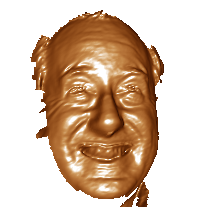
\includegraphics[width=10em]{D1077}} % No eye catcher for this poster. (eyecatcher=no above). If an eye catcher is present, the title is centered between eye-catcher and logo.
  % Title
  {\sf %Sans Serif
  %\bf% Serif
  Expression Invariant Face Recognition with a 3DMM}
  % Authors
  {\sf %Sans Serif
  % Serif
  \vspace{1em}\{Brian.Amberg, Reinhard.Knothe, Thomas.Vetter\}@unibas.ch
  }
  % University logo
  {% The makebox allows the title to flow into the logo, this is a hack because of the L shaped logo.
    \makebox[8em][r]{%
      \begin{minipage}{16em}
        \hfill
        
\includegraphics[height=2em]{msrlogo}
        
\includegraphics[height=7.0em]{logo}
      \end{minipage}
    }
  }

  \tikzstyle{light shaded}=[top color=baposterBGtwo!30!white,bottom color=baposterBGone!30!white,shading=axis,shading angle=30]

  % Width of left inset image
     \setlength{\leftimgwidth}{0.78em+8.0em}

%%%%%%%%%%%%%%%%%%%%%%%%%%%%%%%%%%%%%%%%%%%%%%%%%%%%%%%%%%%%%%%%%%%%%%%%%%%%%%
%%% Now define the boxes that make up the poster
%%%---------------------------------------------------------------------------
%%% Each box has a name and can be placed absolutely or relatively.
%%% The only inconvenience is that you can only specify a relative position 
%%% towards an already declared box. So if you have a box attached to the 
%%% bottom, one to the top and a third one which should be in between, you 
%%% have to specify the top and bottom boxes before you specify the middle 
%%% box.
%%%%%%%%%%%%%%%%%%%%%%%%%%%%%%%%%%%%%%%%%%%%%%%%%%%%%%%%%%%%%%%%%%%%%%%%%%%%%%
    %
    % A coloured circle useful as a bullet with an adjustably strong filling
    \newcommand{\colouredcircle}[1]{%
      \tikz{\useasboundingbox (-0.2em,-0.32em) rectangle(0.2em,0.32em); \draw[draw=black,fill=baposterBGone!80!black!#1!white,line width=0.03em] (0,0) circle(0.18em);}}

%%%%%%%%%%%%%%%%%%%%%%%%%%%%%%%%%%%%%%%%%%%%%%%%%%%%%%%%%%%%%%%%%%%%%%%%%%%%%%
  \headerbox{Contribution}{name=contribution,column=0,row=0}{
%%%%%%%%%%%%%%%%%%%%%%%%%%%%%%%%%%%%%%%%%%%%%%%%%%%%%%%%%%%%%%%%%%%%%%%%%%%%%%
   {}We introduce a method for expression invariant face recognition. A
   generative 3D Morphable Model (3DMM) is used to separate identity and
   expression components. The expression removal results in increased
   recognition performance, even on difficult datasets, without a decrease in
   performance on expression-less datasets.

   It is applicable to any kind of input data, and was evaluated here on
   textureless range scans.
  \vspace{0.3em}
 }

%%%%%%%%%%%%%%%%%%%%%%%%%%%%%%%%%%%%%%%%%%%%%%%%%%%%%%%%%%%%%%%%%%%%%%%%%%%%%%
  \headerbox{Model}{name=model,column=0,below=contribution}{
%%%%%%%%%%%%%%%%%%%%%%%%%%%%%%%%%%%%%%%%%%%%%%%%%%%%%%%%%%%%%%%%%%%%%%%%%%%%%%
    The Model was learnt from 275 subjects. We used one neutral expression scan
    per identity and 150 expression scans of a subset of the subjects. 

    The identity model is a linear model build from the neutral scans.
    \begin{align}
      \VEC f&=\VEC\mu + \MAT M_n\VEC\alpha_n\qquad.
    \end{align}
    For each of the 150 expression scans, we calculated an expression vector as
    the difference between the expression scan and the corresponding neutral
    scan of that subject.  This data is already mode-centered, if we regard the
    neutral expression as the natural mode of expression data. From these offset
    vectors an additional expression matrix $\MAT M_e$ was calculated, such that the complete linear Model is
    \begin{align}
      \VEC f&=\VEC\mu + \MAT M_n\VEC\alpha_n + \MAT M_e\VEC\alpha_e
    \end{align}
    The assumption here is, that the face and expression space are linearly
    independent, such that each face is represented by a unique set of
    coefficients.  
  \vspace{0.3em}
  }

%%%%%%%%%%%%%%%%%%%%%%%%%%%%%%%%%%%%%%%%%%%%%%%%%%%%%%%%%%%%%%%%%%%%%%%%%%%%%%
  \headerbox{Fitting}{name=fitting,column=0,below=model}{
%%%%%%%%%%%%%%%%%%%%%%%%%%%%%%%%%%%%%%%%%%%%%%%%%%%%%%%%%%%%%%%%%%%%%%%%%%%%%%
    A Robust Nonrigid ICP method was used to fit the model to the data.
    Robustness was achieved by iteratively reweighting the correspondences and
    using hard compatability test for the closest points.

    Fitting was initialized by a simple nose detector and proceeded fully
    automatic.
  \vspace{0.3em}
  }

%%%%%%%%%%%%%%%%%%%%%%%%%%%%%%%%%%%%%%%%%%%%%%%%%%%%%%%%%%%%%%%%%%%%%%%%%%%%%%
  \headerbox{Distance Measure}{name=measure,column=0,below=fitting}{
%%%%%%%%%%%%%%%%%%%%%%%%%%%%%%%%%%%%%%%%%%%%%%%%%%%%%%%%%%%%%%%%%%%%%%%%%%%%%%
   The Mahalanobis angle between the identity coefficients $\VEC{\alpha_{n}}$
   was used for classification.
  \vspace{0.3em}
  }

%%%%%%%%%%%%%%%%%%%%%%%%%%%%%%%%%%%%%%%%%%%%%%%%%%%%%%%%%%%%%%%%%%%%%%%%%%%%%%
  \headerbox{Expression Neutralization}{name=results neutralization,column=1,row=0}{
%%%%%%%%%%%%%%%%%%%%%%%%%%%%%%%%%%%%%%%%%%%%%%%%%%%%%%%%%%%%%%%%%%%%%%%%%%%%%%
  \begin{tikzpicture}[x=0.3333\linewidth,y=-0.42\linewidth]
    \path [use as bounding box] (-0.5,-0.5) rectangle(2.5,1.7);
    \path
    (0,0) node{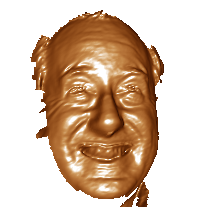
\includegraphics[width=0.42\linewidth]{D1077}}
    (1,0) node{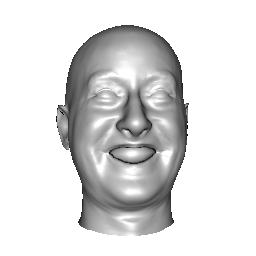
\includegraphics[width=0.47\linewidth]{D1077_fit_expression}}
    (2,0) node{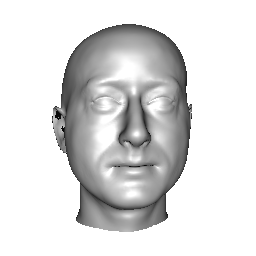
\includegraphics[width=0.47\linewidth]{D1077_fit}}

    (0,1) node{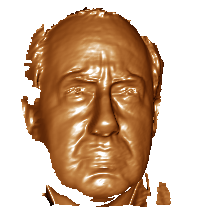
\includegraphics[width=0.42\linewidth]{D1360}}
    (1,1) node{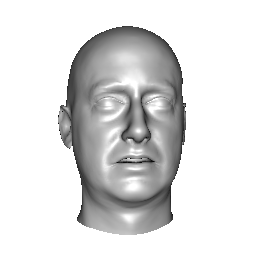
\includegraphics[width=0.47\linewidth]{D1360_fit_expression}}
    (2,1) node{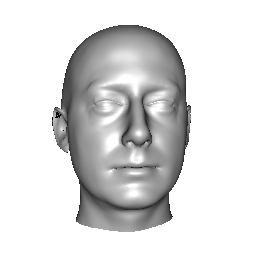
\includegraphics[width=0.47\linewidth]{D1360_fit}}

    (0,1.6) node {\smaller a) Target}
    (1,1.6) node {\smaller b) Fit}
    (2,1.6) node {\smaller c) Normalized};
  \end{tikzpicture}
  \vspace{0.5em}

  Expression normalisation for two scans of the same individual.  
  The robust fitting gives a good estimate (b) of the true face surface given
  the noisy measurement (a). It fills in holes and removes artifacts using
  prior knowledge from the face model. The pose and expression normalized faces
  (c) are used for face recognition.
  \vspace{0.5em}
  }
%%%%%%%%%%%%%%%%%%%%%%%%%%%%%%%%%%%%%%%%%%%%%%%%%%%%%%%%%%%%%%%%%%%%%%%%%%%%%%
  \headerbox{Funding}{name=funding,column=1,span=2,above=bottom}{
%%%%%%%%%%%%%%%%%%%%%%%%%%%%%%%%%%%%%%%%%%%%%%%%%%%%%%%%%%%%%%%%%%%%%%%%%%%%%%
  \smaller 
  \hspace{1em}This work was supported in part by Microsoft Research through the European PhD Scholarship Programme.
  }
%%%%%%%%%%%%%%%%%%%%%%%%%%%%%%%%%%%%%%%%%%%%%%%%%%%%%%%%%%%%%%%%%%%%%%%%%%%%%%
  \headerbox{Results}{name=results,column=1,span=2,below=results neutralization,above=funding}{
%%%%%%%%%%%%%%%%%%%%%%%%%%%%%%%%%%%%%%%%%%%%%%%%%%%%%%%%%%%%%%%%%%%%%%%%%%%%%%
      \begin{multicols}{2}
        The method was evaluated on the GavabDB expression dataset which
        contains 427 Scans, with 3 neutral scans and 4 expression scans per ID.
        To test the impact of expression invariance on neutral data we used the
        UND Dataset from the Face Recognition Great Vendor Test, which contains
        953 neutral scans with one to eight scans per subject.
      \end{multicols}\vspace{-1em}
      \mbox{\hspace{0.3\linewidth}\rule{0.4\linewidth}{1pt}\hspace{0.3\linewidth}}\\
      \begin{tabular}{cc}
        \hspace{-0.5em}\scalebox{0.735}{\input{shrec_mncg}} &
        \hspace{0.5em}\scalebox{0.735}{% GNUPLOT: LaTeX picture with Postscript
\begingroup
  \fontfamily{phv}%
  \selectfont
  \makeatletter
  \providecommand\color[2][]{%
    \GenericError{(gnuplot) \space\space\space\@spaces}{%
      Package color not loaded in conjunction with
      terminal option `colourtext'%
    }{See the gnuplot documentation for explanation.%
    }{Either use 'blacktext' in gnuplot or load the package
      color.sty in LaTeX.}%
    \renewcommand\color[2][]{}%
  }%
  \providecommand\includegraphics[2][]{%
    \GenericError{(gnuplot) \space\space\space\@spaces}{%
      Package graphicx or graphics not loaded%
    }{See the gnuplot documentation for explanation.%
    }{The gnuplot epslatex terminal needs graphicx.sty or graphics.sty.}%
    \renewcommand\includegraphics[2][]{}%
  }%
  \providecommand\rotatebox[2]{#2}%
  \@ifundefined{ifGPcolor}{%
    \newif\ifGPcolor
    \GPcolortrue
  }{}%
  \@ifundefined{ifGPblacktext}{%
    \newif\ifGPblacktext
    \GPblacktextfalse
  }{}%
  % define a \g@addto@macro without @ in the name:
  \let\gplgaddtomacro\g@addto@macro
  % define empty templates for all commands taking text:
  \gdef\gplbacktext{}%
  \gdef\gplfronttext{}%
  \makeatother
  \ifGPblacktext
    % no textcolor at all
    \def\colorrgb#1{}%
    \def\colorgray#1{}%
  \else
    % gray or color?
    \ifGPcolor
      \def\colorrgb#1{\color[rgb]{#1}}%
      \def\colorgray#1{\color[gray]{#1}}%
      \expandafter\def\csname LTw\endcsname{\color{white}}%
      \expandafter\def\csname LTb\endcsname{\color{black}}%
      \expandafter\def\csname LTa\endcsname{\color{black}}%
      \expandafter\def\csname LT0\endcsname{\color[rgb]{1,0,0}}%
      \expandafter\def\csname LT1\endcsname{\color[rgb]{0,1,0}}%
      \expandafter\def\csname LT2\endcsname{\color[rgb]{0,0,1}}%
      \expandafter\def\csname LT3\endcsname{\color[rgb]{1,0,1}}%
      \expandafter\def\csname LT4\endcsname{\color[rgb]{0,1,1}}%
      \expandafter\def\csname LT5\endcsname{\color[rgb]{1,1,0}}%
      \expandafter\def\csname LT6\endcsname{\color[rgb]{0,0,0}}%
      \expandafter\def\csname LT7\endcsname{\color[rgb]{1,0.3,0}}%
      \expandafter\def\csname LT8\endcsname{\color[rgb]{0.5,0.5,0.5}}%
    \else
      % gray
      \def\colorrgb#1{\color{black}}%
      \def\colorgray#1{\color[gray]{#1}}%
      \expandafter\def\csname LTw\endcsname{\color{white}}%
      \expandafter\def\csname LTb\endcsname{\color{black}}%
      \expandafter\def\csname LTa\endcsname{\color{black}}%
      \expandafter\def\csname LT0\endcsname{\color{black}}%
      \expandafter\def\csname LT1\endcsname{\color{black}}%
      \expandafter\def\csname LT2\endcsname{\color{black}}%
      \expandafter\def\csname LT3\endcsname{\color{black}}%
      \expandafter\def\csname LT4\endcsname{\color{black}}%
      \expandafter\def\csname LT5\endcsname{\color{black}}%
      \expandafter\def\csname LT6\endcsname{\color{black}}%
      \expandafter\def\csname LT7\endcsname{\color{black}}%
      \expandafter\def\csname LT8\endcsname{\color{black}}%
    \fi
  \fi
  \setlength{\unitlength}{0.0500bp}%
  \begin{picture}(5760.00,2520.00)%
    \gplgaddtomacro\gplbacktext{%
      \csname LTb\endcsname%
      \put(1026,540){\makebox(0,0)[r]{\strut{} 0.99}}%
      \csname LTb\endcsname%
      \put(1026,828){\makebox(0,0)[r]{\strut{} 0.992}}%
      \csname LTb\endcsname%
      \put(1026,1116){\makebox(0,0)[r]{\strut{} 0.994}}%
      \csname LTb\endcsname%
      \put(1026,1404){\makebox(0,0)[r]{\strut{} 0.996}}%
      \csname LTb\endcsname%
      \put(1026,1692){\makebox(0,0)[r]{\strut{} 0.998}}%
      \csname LTb\endcsname%
      \put(1026,1980){\makebox(0,0)[r]{\strut{} 1}}%
      \csname LTb\endcsname%
      \put(1134,360){\makebox(0,0){\strut{} 0}}%
      \csname LTb\endcsname%
      \put(1566,360){\makebox(0,0){\strut{} 2}}%
      \csname LTb\endcsname%
      \put(1998,360){\makebox(0,0){\strut{} 4}}%
      \csname LTb\endcsname%
      \put(2430,360){\makebox(0,0){\strut{} 6}}%
      \csname LTb\endcsname%
      \put(2862,360){\makebox(0,0){\strut{} 8}}%
      \csname LTb\endcsname%
      \put(3294,360){\makebox(0,0){\strut{} 10}}%
      \csname LTb\endcsname%
      \put(3726,360){\makebox(0,0){\strut{} 12}}%
      \csname LTb\endcsname%
      \put(4158,360){\makebox(0,0){\strut{} 14}}%
      \csname LTb\endcsname%
      \put(4590,360){\makebox(0,0){\strut{} 16}}%
      \csname LTb\endcsname%
      \put(5022,360){\makebox(0,0){\strut{} 18}}%
      \csname LTb\endcsname%
      \put(5454,360){\makebox(0,0){\strut{} 20}}%
      \put(180,1260){\rotatebox{90}{\makebox(0,0){\strut{}MNCG}}}%
      \put(3294,90){\makebox(0,0){\strut{}$@x$}}%
      \put(3294,2250){\makebox(0,0){\strut{}UND: Mean Normalized Cumulative Gain}}%
    }%
    \gplgaddtomacro\gplfronttext{%
      \csname LTb\endcsname%
      \put(4635,873){\makebox(0,0)[r]{\strut{}neutral model}}%
      \csname LTb\endcsname%
      \put(4635,693){\makebox(0,0)[r]{\strut{}expression model}}%
    }%
    \gplbacktext
    \put(0,0){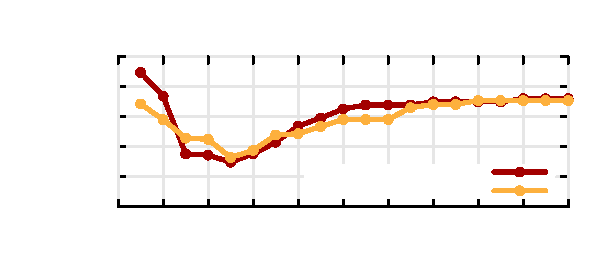
\includegraphics{und_MNCG}}%
    \gplfronttext
  \end{picture}%
\endgroup
}
      \end{tabular}\\
%      \begin{multicols}{2}
        {Expression neutralization improves results on the expression dataset
        without decreasing the accuracy on the neutral testset. Plotted is the
        ratio of correct answers to  the number of possible correct answers.
        %Note the different scales for the two graphs.
        %Our approach has a high accuracy on the neutral (UND) dataset.
        }
%      \end{multicols}\vspace{-1em}
      \\\mbox{\hspace{0.3\linewidth}\rule{0.4\linewidth}{1pt}\hspace{0.3\linewidth}}\\
      \begin{tabular}{cc}
        \hspace{-0.5em}\scalebox{0.735}{% GNUPLOT: LaTeX picture with Postscript
\begingroup
  \fontfamily{phv}%
  \selectfont
  \makeatletter
  \providecommand\color[2][]{%
    \GenericError{(gnuplot) \space\space\space\@spaces}{%
      Package color not loaded in conjunction with
      terminal option `colourtext'%
    }{See the gnuplot documentation for explanation.%
    }{Either use 'blacktext' in gnuplot or load the package
      color.sty in LaTeX.}%
    \renewcommand\color[2][]{}%
  }%
  \providecommand\includegraphics[2][]{%
    \GenericError{(gnuplot) \space\space\space\@spaces}{%
      Package graphicx or graphics not loaded%
    }{See the gnuplot documentation for explanation.%
    }{The gnuplot epslatex terminal needs graphicx.sty or graphics.sty.}%
    \renewcommand\includegraphics[2][]{}%
  }%
  \providecommand\rotatebox[2]{#2}%
  \@ifundefined{ifGPcolor}{%
    \newif\ifGPcolor
    \GPcolortrue
  }{}%
  \@ifundefined{ifGPblacktext}{%
    \newif\ifGPblacktext
    \GPblacktextfalse
  }{}%
  % define a \g@addto@macro without @ in the name:
  \let\gplgaddtomacro\g@addto@macro
  % define empty templates for all commands taking text:
  \gdef\gplbacktext{}%
  \gdef\gplfronttext{}%
  \makeatother
  \ifGPblacktext
    % no textcolor at all
    \def\colorrgb#1{}%
    \def\colorgray#1{}%
  \else
    % gray or color?
    \ifGPcolor
      \def\colorrgb#1{\color[rgb]{#1}}%
      \def\colorgray#1{\color[gray]{#1}}%
      \expandafter\def\csname LTw\endcsname{\color{white}}%
      \expandafter\def\csname LTb\endcsname{\color{black}}%
      \expandafter\def\csname LTa\endcsname{\color{black}}%
      \expandafter\def\csname LT0\endcsname{\color[rgb]{1,0,0}}%
      \expandafter\def\csname LT1\endcsname{\color[rgb]{0,1,0}}%
      \expandafter\def\csname LT2\endcsname{\color[rgb]{0,0,1}}%
      \expandafter\def\csname LT3\endcsname{\color[rgb]{1,0,1}}%
      \expandafter\def\csname LT4\endcsname{\color[rgb]{0,1,1}}%
      \expandafter\def\csname LT5\endcsname{\color[rgb]{1,1,0}}%
      \expandafter\def\csname LT6\endcsname{\color[rgb]{0,0,0}}%
      \expandafter\def\csname LT7\endcsname{\color[rgb]{1,0.3,0}}%
      \expandafter\def\csname LT8\endcsname{\color[rgb]{0.5,0.5,0.5}}%
    \else
      % gray
      \def\colorrgb#1{\color{black}}%
      \def\colorgray#1{\color[gray]{#1}}%
      \expandafter\def\csname LTw\endcsname{\color{white}}%
      \expandafter\def\csname LTb\endcsname{\color{black}}%
      \expandafter\def\csname LTa\endcsname{\color{black}}%
      \expandafter\def\csname LT0\endcsname{\color{black}}%
      \expandafter\def\csname LT1\endcsname{\color{black}}%
      \expandafter\def\csname LT2\endcsname{\color{black}}%
      \expandafter\def\csname LT3\endcsname{\color{black}}%
      \expandafter\def\csname LT4\endcsname{\color{black}}%
      \expandafter\def\csname LT5\endcsname{\color{black}}%
      \expandafter\def\csname LT6\endcsname{\color{black}}%
      \expandafter\def\csname LT7\endcsname{\color{black}}%
      \expandafter\def\csname LT8\endcsname{\color{black}}%
    \fi
  \fi
  \setlength{\unitlength}{0.0500bp}%
  \begin{picture}(5760.00,2520.00)%
    \gplgaddtomacro\gplbacktext{%
      \csname LTb\endcsname%
      \put(810,540){\makebox(0,0)[r]{\strut{} 0}}%
      \csname LTb\endcsname%
      \put(810,828){\makebox(0,0)[r]{\strut{} 0.2}}%
      \csname LTb\endcsname%
      \put(810,1116){\makebox(0,0)[r]{\strut{} 0.4}}%
      \csname LTb\endcsname%
      \put(810,1404){\makebox(0,0)[r]{\strut{} 0.6}}%
      \csname LTb\endcsname%
      \put(810,1692){\makebox(0,0)[r]{\strut{} 0.8}}%
      \csname LTb\endcsname%
      \put(810,1980){\makebox(0,0)[r]{\strut{} 1}}%
      \csname LTb\endcsname%
      \put(918,360){\makebox(0,0){\strut{} 0}}%
      \csname LTb\endcsname%
      \put(1825,360){\makebox(0,0){\strut{} 0.2}}%
      \csname LTb\endcsname%
      \put(2732,360){\makebox(0,0){\strut{} 0.4}}%
      \csname LTb\endcsname%
      \put(3640,360){\makebox(0,0){\strut{} 0.6}}%
      \csname LTb\endcsname%
      \put(4547,360){\makebox(0,0){\strut{} 0.8}}%
      \csname LTb\endcsname%
      \put(5454,360){\makebox(0,0){\strut{} 1}}%
      \put(180,1260){\rotatebox{90}{\makebox(0,0){\strut{}Precision}}}%
      \put(3186,90){\makebox(0,0){\strut{}Recall}}%
      \put(3186,2250){\makebox(0,0){\strut{}GavabDB: Precision Recall}}%
    }%
    \gplgaddtomacro\gplfronttext{%
      \csname LTb\endcsname%
      \put(2754,873){\makebox(0,0)[r]{\strut{}neutral model}}%
      \csname LTb\endcsname%
      \put(2754,693){\makebox(0,0)[r]{\strut{}expression model}}%
    }%
    \gplbacktext
    \put(0,0){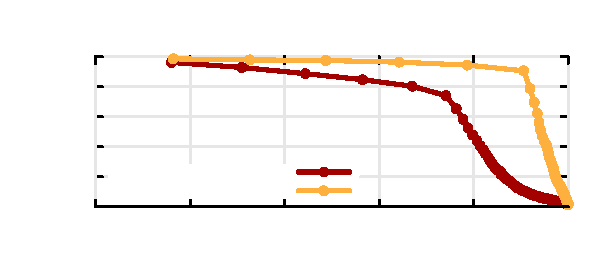
\includegraphics{shrec_PR}}%
    \gplfronttext
  \end{picture}%
\endgroup
} &
        \hspace{0.5em}\scalebox{0.735}{% GNUPLOT: LaTeX picture with Postscript
\begingroup
  \fontfamily{phv}%
  \selectfont
  \makeatletter
  \providecommand\color[2][]{%
    \GenericError{(gnuplot) \space\space\space\@spaces}{%
      Package color not loaded in conjunction with
      terminal option `colourtext'%
    }{See the gnuplot documentation for explanation.%
    }{Either use 'blacktext' in gnuplot or load the package
      color.sty in LaTeX.}%
    \renewcommand\color[2][]{}%
  }%
  \providecommand\includegraphics[2][]{%
    \GenericError{(gnuplot) \space\space\space\@spaces}{%
      Package graphicx or graphics not loaded%
    }{See the gnuplot documentation for explanation.%
    }{The gnuplot epslatex terminal needs graphicx.sty or graphics.sty.}%
    \renewcommand\includegraphics[2][]{}%
  }%
  \providecommand\rotatebox[2]{#2}%
  \@ifundefined{ifGPcolor}{%
    \newif\ifGPcolor
    \GPcolortrue
  }{}%
  \@ifundefined{ifGPblacktext}{%
    \newif\ifGPblacktext
    \GPblacktextfalse
  }{}%
  % define a \g@addto@macro without @ in the name:
  \let\gplgaddtomacro\g@addto@macro
  % define empty templates for all commands taking text:
  \gdef\gplbacktext{}%
  \gdef\gplfronttext{}%
  \makeatother
  \ifGPblacktext
    % no textcolor at all
    \def\colorrgb#1{}%
    \def\colorgray#1{}%
  \else
    % gray or color?
    \ifGPcolor
      \def\colorrgb#1{\color[rgb]{#1}}%
      \def\colorgray#1{\color[gray]{#1}}%
      \expandafter\def\csname LTw\endcsname{\color{white}}%
      \expandafter\def\csname LTb\endcsname{\color{black}}%
      \expandafter\def\csname LTa\endcsname{\color{black}}%
      \expandafter\def\csname LT0\endcsname{\color[rgb]{1,0,0}}%
      \expandafter\def\csname LT1\endcsname{\color[rgb]{0,1,0}}%
      \expandafter\def\csname LT2\endcsname{\color[rgb]{0,0,1}}%
      \expandafter\def\csname LT3\endcsname{\color[rgb]{1,0,1}}%
      \expandafter\def\csname LT4\endcsname{\color[rgb]{0,1,1}}%
      \expandafter\def\csname LT5\endcsname{\color[rgb]{1,1,0}}%
      \expandafter\def\csname LT6\endcsname{\color[rgb]{0,0,0}}%
      \expandafter\def\csname LT7\endcsname{\color[rgb]{1,0.3,0}}%
      \expandafter\def\csname LT8\endcsname{\color[rgb]{0.5,0.5,0.5}}%
    \else
      % gray
      \def\colorrgb#1{\color{black}}%
      \def\colorgray#1{\color[gray]{#1}}%
      \expandafter\def\csname LTw\endcsname{\color{white}}%
      \expandafter\def\csname LTb\endcsname{\color{black}}%
      \expandafter\def\csname LTa\endcsname{\color{black}}%
      \expandafter\def\csname LT0\endcsname{\color{black}}%
      \expandafter\def\csname LT1\endcsname{\color{black}}%
      \expandafter\def\csname LT2\endcsname{\color{black}}%
      \expandafter\def\csname LT3\endcsname{\color{black}}%
      \expandafter\def\csname LT4\endcsname{\color{black}}%
      \expandafter\def\csname LT5\endcsname{\color{black}}%
      \expandafter\def\csname LT6\endcsname{\color{black}}%
      \expandafter\def\csname LT7\endcsname{\color{black}}%
      \expandafter\def\csname LT8\endcsname{\color{black}}%
    \fi
  \fi
  \setlength{\unitlength}{0.0500bp}%
  \begin{picture}(5760.00,2520.00)%
    \gplgaddtomacro\gplbacktext{%
      \csname LTb\endcsname%
      \put(810,540){\makebox(0,0)[r]{\strut{} 0}}%
      \csname LTb\endcsname%
      \put(810,828){\makebox(0,0)[r]{\strut{} 0.2}}%
      \csname LTb\endcsname%
      \put(810,1116){\makebox(0,0)[r]{\strut{} 0.4}}%
      \csname LTb\endcsname%
      \put(810,1404){\makebox(0,0)[r]{\strut{} 0.6}}%
      \csname LTb\endcsname%
      \put(810,1692){\makebox(0,0)[r]{\strut{} 0.8}}%
      \csname LTb\endcsname%
      \put(810,1980){\makebox(0,0)[r]{\strut{} 1}}%
      \csname LTb\endcsname%
      \put(918,360){\makebox(0,0){\strut{} 0}}%
      \csname LTb\endcsname%
      \put(1825,360){\makebox(0,0){\strut{} 0.2}}%
      \csname LTb\endcsname%
      \put(2732,360){\makebox(0,0){\strut{} 0.4}}%
      \csname LTb\endcsname%
      \put(3640,360){\makebox(0,0){\strut{} 0.6}}%
      \csname LTb\endcsname%
      \put(4547,360){\makebox(0,0){\strut{} 0.8}}%
      \csname LTb\endcsname%
      \put(5454,360){\makebox(0,0){\strut{} 1}}%
      \put(180,1260){\rotatebox{90}{\makebox(0,0){\strut{}Precision}}}%
      \put(3186,90){\makebox(0,0){\strut{}Recall}}%
      \put(3186,2250){\makebox(0,0){\strut{}UND: Precision Recall}}%
    }%
    \gplgaddtomacro\gplfronttext{%
      \csname LTb\endcsname%
      \put(2754,873){\makebox(0,0)[r]{\strut{}neutral model}}%
      \csname LTb\endcsname%
      \put(2754,693){\makebox(0,0)[r]{\strut{}expression model}}%
    }%
    \gplbacktext
    \put(0,0){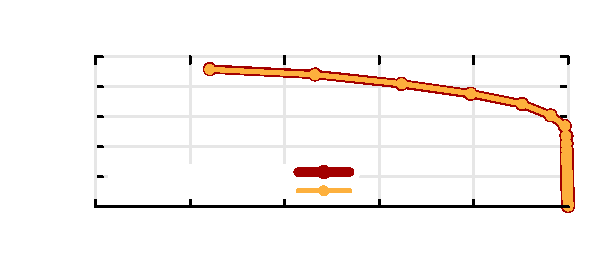
\includegraphics{und_PR}}%
    \gplfronttext
  \end{picture}%
\endgroup
}
      \end{tabular}\\
%      \begin{multicols}{2}
        {Plotted are precision and recall for different retrieval depths. The lower
        precision of the UND database is due to the fact that some queries have no
        correct answers.}
%      \end{multicols}\vspace{-1em}
      \\\mbox{\hspace{0.3\linewidth}\rule{0.4\linewidth}{1pt}\hspace{0.3\linewidth}}\\
      \begin{tabular}{cc}
        \hspace{-0.5em}\scalebox{0.735}{% GNUPLOT: LaTeX picture with Postscript
\begingroup
  \fontfamily{phv}%
  \selectfont
  \makeatletter
  \providecommand\color[2][]{%
    \GenericError{(gnuplot) \space\space\space\@spaces}{%
      Package color not loaded in conjunction with
      terminal option `colourtext'%
    }{See the gnuplot documentation for explanation.%
    }{Either use 'blacktext' in gnuplot or load the package
      color.sty in LaTeX.}%
    \renewcommand\color[2][]{}%
  }%
  \providecommand\includegraphics[2][]{%
    \GenericError{(gnuplot) \space\space\space\@spaces}{%
      Package graphicx or graphics not loaded%
    }{See the gnuplot documentation for explanation.%
    }{The gnuplot epslatex terminal needs graphicx.sty or graphics.sty.}%
    \renewcommand\includegraphics[2][]{}%
  }%
  \providecommand\rotatebox[2]{#2}%
  \@ifundefined{ifGPcolor}{%
    \newif\ifGPcolor
    \GPcolortrue
  }{}%
  \@ifundefined{ifGPblacktext}{%
    \newif\ifGPblacktext
    \GPblacktexttrue
  }{}%
  % define a \g@addto@macro without @ in the name:
  \let\gplgaddtomacro\g@addto@macro
  % define empty templates for all commands taking text:
  \gdef\gplbacktext{}%
  \gdef\gplfronttext{}%
  \makeatother
  \ifGPblacktext
    % no textcolor at all
    \def\colorrgb#1{}%
    \def\colorgray#1{}%
  \else
    % gray or color?
    \ifGPcolor
      \def\colorrgb#1{\color[rgb]{#1}}%
      \def\colorgray#1{\color[gray]{#1}}%
      \expandafter\def\csname LTw\endcsname{\color{white}}%
      \expandafter\def\csname LTb\endcsname{\color{black}}%
      \expandafter\def\csname LTa\endcsname{\color{black}}%
      \expandafter\def\csname LT0\endcsname{\color[rgb]{1,0,0}}%
      \expandafter\def\csname LT1\endcsname{\color[rgb]{0,1,0}}%
      \expandafter\def\csname LT2\endcsname{\color[rgb]{0,0,1}}%
      \expandafter\def\csname LT3\endcsname{\color[rgb]{1,0,1}}%
      \expandafter\def\csname LT4\endcsname{\color[rgb]{0,1,1}}%
      \expandafter\def\csname LT5\endcsname{\color[rgb]{1,1,0}}%
      \expandafter\def\csname LT6\endcsname{\color[rgb]{0,0,0}}%
      \expandafter\def\csname LT7\endcsname{\color[rgb]{1,0.3,0}}%
      \expandafter\def\csname LT8\endcsname{\color[rgb]{0.5,0.5,0.5}}%
    \else
      % gray
      \def\colorrgb#1{\color{black}}%
      \def\colorgray#1{\color[gray]{#1}}%
      \expandafter\def\csname LTw\endcsname{\color{white}}%
      \expandafter\def\csname LTb\endcsname{\color{black}}%
      \expandafter\def\csname LTa\endcsname{\color{black}}%
      \expandafter\def\csname LT0\endcsname{\color{black}}%
      \expandafter\def\csname LT1\endcsname{\color{black}}%
      \expandafter\def\csname LT2\endcsname{\color{black}}%
      \expandafter\def\csname LT3\endcsname{\color{black}}%
      \expandafter\def\csname LT4\endcsname{\color{black}}%
      \expandafter\def\csname LT5\endcsname{\color{black}}%
      \expandafter\def\csname LT6\endcsname{\color{black}}%
      \expandafter\def\csname LT7\endcsname{\color{black}}%
      \expandafter\def\csname LT8\endcsname{\color{black}}%
    \fi
  \fi
  \setlength{\unitlength}{0.0500bp}%
  \begin{picture}(5760.00,2520.00)%
    \gplgaddtomacro\gplbacktext{%
      \csname LTb\endcsname%
      \put(810,540){\makebox(0,0)[r]{\strut{} 0}}%
      \csname LTb\endcsname%
      \put(810,900){\makebox(0,0)[r]{\strut{} 0.5}}%
      \csname LTb\endcsname%
      \put(810,1260){\makebox(0,0)[r]{\strut{} 1}}%
      \csname LTb\endcsname%
      \put(810,1620){\makebox(0,0)[r]{\strut{} 1.5}}%
      \csname LTb\endcsname%
      \put(810,1980){\makebox(0,0)[r]{\strut{} 2}}%
      \csname LTb\endcsname%
      \put(918,360){\makebox(0,0){\strut{} 0}}%
      \csname LTb\endcsname%
      \put(1825,360){\makebox(0,0){\strut{} 0.2}}%
      \csname LTb\endcsname%
      \put(2732,360){\makebox(0,0){\strut{} 0.4}}%
      \csname LTb\endcsname%
      \put(3640,360){\makebox(0,0){\strut{} 0.6}}%
      \csname LTb\endcsname%
      \put(4547,360){\makebox(0,0){\strut{} 0.8}}%
      \csname LTb\endcsname%
      \put(5454,360){\makebox(0,0){\strut{} 1}}%
      \put(180,1260){\rotatebox{90}{\makebox(0,0){\strut{}FRR \%}}}%
      \put(3186,90){\makebox(0,0){\strut{}FAR \%}}%
      \put(3186,2250){\makebox(0,0){\strut{}\bf \normalsize GavabDB: Recognition Performance}}%
    }%
    \gplgaddtomacro\gplfronttext{%
      \csname LTb\endcsname%
      \put(4635,1827){\makebox(0,0)[r]{\strut{}neutral model}}%
      \csname LTb\endcsname%
      \put(4635,1647){\makebox(0,0)[r]{\strut{}expression model}}%
    }%
    \gplbacktext
    \put(0,0){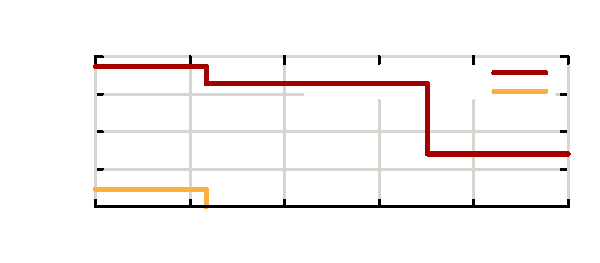
\includegraphics{shrec_far_frr}}%
    \gplfronttext
  \end{picture}%
\endgroup
} &
        \hspace{0.5em}\scalebox{0.735}{% GNUPLOT: LaTeX picture with Postscript
\begingroup
  \fontfamily{phv}%
  \selectfont
  \makeatletter
  \providecommand\color[2][]{%
    \GenericError{(gnuplot) \space\space\space\@spaces}{%
      Package color not loaded in conjunction with
      terminal option `colourtext'%
    }{See the gnuplot documentation for explanation.%
    }{Either use 'blacktext' in gnuplot or load the package
      color.sty in LaTeX.}%
    \renewcommand\color[2][]{}%
  }%
  \providecommand\includegraphics[2][]{%
    \GenericError{(gnuplot) \space\space\space\@spaces}{%
      Package graphicx or graphics not loaded%
    }{See the gnuplot documentation for explanation.%
    }{The gnuplot epslatex terminal needs graphicx.sty or graphics.sty.}%
    \renewcommand\includegraphics[2][]{}%
  }%
  \providecommand\rotatebox[2]{#2}%
  \@ifundefined{ifGPcolor}{%
    \newif\ifGPcolor
    \GPcolortrue
  }{}%
  \@ifundefined{ifGPblacktext}{%
    \newif\ifGPblacktext
    \GPblacktexttrue
  }{}%
  % define a \g@addto@macro without @ in the name:
  \let\gplgaddtomacro\g@addto@macro
  % define empty templates for all commands taking text:
  \gdef\gplbacktext{}%
  \gdef\gplfronttext{}%
  \makeatother
  \ifGPblacktext
    % no textcolor at all
    \def\colorrgb#1{}%
    \def\colorgray#1{}%
  \else
    % gray or color?
    \ifGPcolor
      \def\colorrgb#1{\color[rgb]{#1}}%
      \def\colorgray#1{\color[gray]{#1}}%
      \expandafter\def\csname LTw\endcsname{\color{white}}%
      \expandafter\def\csname LTb\endcsname{\color{black}}%
      \expandafter\def\csname LTa\endcsname{\color{black}}%
      \expandafter\def\csname LT0\endcsname{\color[rgb]{1,0,0}}%
      \expandafter\def\csname LT1\endcsname{\color[rgb]{0,1,0}}%
      \expandafter\def\csname LT2\endcsname{\color[rgb]{0,0,1}}%
      \expandafter\def\csname LT3\endcsname{\color[rgb]{1,0,1}}%
      \expandafter\def\csname LT4\endcsname{\color[rgb]{0,1,1}}%
      \expandafter\def\csname LT5\endcsname{\color[rgb]{1,1,0}}%
      \expandafter\def\csname LT6\endcsname{\color[rgb]{0,0,0}}%
      \expandafter\def\csname LT7\endcsname{\color[rgb]{1,0.3,0}}%
      \expandafter\def\csname LT8\endcsname{\color[rgb]{0.5,0.5,0.5}}%
    \else
      % gray
      \def\colorrgb#1{\color{black}}%
      \def\colorgray#1{\color[gray]{#1}}%
      \expandafter\def\csname LTw\endcsname{\color{white}}%
      \expandafter\def\csname LTb\endcsname{\color{black}}%
      \expandafter\def\csname LTa\endcsname{\color{black}}%
      \expandafter\def\csname LT0\endcsname{\color{black}}%
      \expandafter\def\csname LT1\endcsname{\color{black}}%
      \expandafter\def\csname LT2\endcsname{\color{black}}%
      \expandafter\def\csname LT3\endcsname{\color{black}}%
      \expandafter\def\csname LT4\endcsname{\color{black}}%
      \expandafter\def\csname LT5\endcsname{\color{black}}%
      \expandafter\def\csname LT6\endcsname{\color{black}}%
      \expandafter\def\csname LT7\endcsname{\color{black}}%
      \expandafter\def\csname LT8\endcsname{\color{black}}%
    \fi
  \fi
  \setlength{\unitlength}{0.0500bp}%
  \begin{picture}(5760.00,2520.00)%
    \gplgaddtomacro\gplbacktext{%
      \csname LTb\endcsname%
      \put(810,540){\makebox(0,0)[r]{\strut{} 0}}%
      \csname LTb\endcsname%
      \put(810,900){\makebox(0,0)[r]{\strut{} 0.5}}%
      \csname LTb\endcsname%
      \put(810,1260){\makebox(0,0)[r]{\strut{} 1}}%
      \csname LTb\endcsname%
      \put(810,1620){\makebox(0,0)[r]{\strut{} 1.5}}%
      \csname LTb\endcsname%
      \put(810,1980){\makebox(0,0)[r]{\strut{} 2}}%
      \csname LTb\endcsname%
      \put(918,360){\makebox(0,0){\strut{} 0}}%
      \csname LTb\endcsname%
      \put(1825,360){\makebox(0,0){\strut{} 0.2}}%
      \csname LTb\endcsname%
      \put(2732,360){\makebox(0,0){\strut{} 0.4}}%
      \csname LTb\endcsname%
      \put(3640,360){\makebox(0,0){\strut{} 0.6}}%
      \csname LTb\endcsname%
      \put(4547,360){\makebox(0,0){\strut{} 0.8}}%
      \csname LTb\endcsname%
      \put(5454,360){\makebox(0,0){\strut{} 1}}%
      \put(180,1260){\rotatebox{90}{\makebox(0,0){\strut{}FRR \%}}}%
      \put(3186,90){\makebox(0,0){\strut{}FAR \%}}%
      \put(3186,2250){\makebox(0,0){\strut{}\bf \normalsize UND: Recognition Performance}}%
    }%
    \gplgaddtomacro\gplfronttext{%
      \csname LTb\endcsname%
      \put(4635,1827){\makebox(0,0)[r]{\strut{}neutral model}}%
      \csname LTb\endcsname%
      \put(4635,1647){\makebox(0,0)[r]{\strut{}expression model}}%
    }%
    \gplbacktext
    \put(0,0){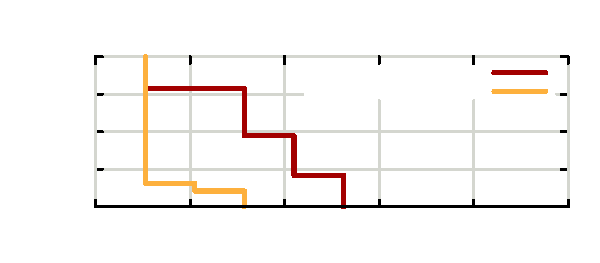
\includegraphics{und_far_frr}}%
    \gplfronttext
  \end{picture}%
\endgroup
}
      \end{tabular}\\
%      \begin{multicols}{2}
        {Impostor detection is reliable, as the minimum distance to a match
        is smaller than the minimum distance to a nonmatch. }
%      \end{multicols}
  \\
  \vspace{0.5em}
  }
%%%%%%%%%%%%%%%%%%%%%%%%%%%%%%%%%%%%%%%%%%%%%%%%%%%%%%%%%%%%%%%%%%%%%%%%%%%%%%
  \headerbox{Robustness}{name=robustness,column=2,row=0,above=results,span=1}{
%%%%%%%%%%%%%%%%%%%%%%%%%%%%%%%%%%%%%%%%%%%%%%%%%%%%%%%%%%%%%%%%%%%%%%%%%%%%%%
  \begin{tikzpicture}[x=0.3333\linewidth,y=-0.42\linewidth]
    \path [use as bounding box] (-0.5,-0.5) rectangle(2.5,1.7);
    \path
    (0,0) node{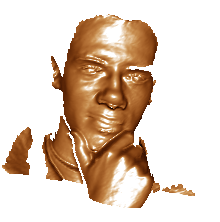
\includegraphics[width=0.42\linewidth]{D1160}}
    (1,0) node{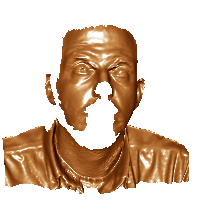
\includegraphics[width=0.42\linewidth]{D1425}}
    (2,0) node{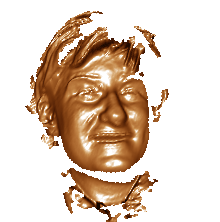
\includegraphics[width=0.42\linewidth]{D1205}}

    (0,1) node{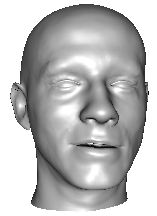
\includegraphics[width=0.28\linewidth]{D1160_fit_expression}}
    (1,1) node{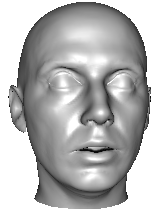
\includegraphics[width=0.28\linewidth]{D1425_fit_expression}}
    (2,1) node{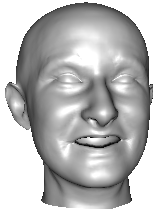
\includegraphics[width=0.28\linewidth]{D1205_fit_expression}}

    (1,0.5) node {\smaller a) Target}
    (1,1.6) node {\smaller b) Robust Reconstruction};
  \end{tikzpicture}
  \vspace{0.5em}

  The reconstruction (b) is robust against scans (a) with artifacts, noise, and
  holes.
  
  This is achieved by a robust iteratively reweighted ICP algorithm and outlier
  rejection based on angle comparisions between corresponding points.
  }

%%%%%%%%%%%%%%%%%%%%%%%%%%%%%%%%%%%%%%%%%%%%%%%%%%%%%%%%%%%%%%%%%%%%%%%%%%%%%%
  \headerbox{References}{name=references,column=0,above=bottom}{
%%%%%%%%%%%%%%%%%%%%%%%%%%%%%%%%%%%%%%%%%%%%%%%%%%%%%%%%%%%%%%%%%%%%%%%%%%%%%%
    \smaller
    \vspace{-0.4em}
    \bibliographystyle{ieee}
    \renewcommand{\section}[2]{\vskip 0.05em}
      \begin{thebibliography}{1}\itemsep=-0.01em
      \setlength{\baselineskip}{0.4em}
      \bibitem{amberg07:nonrigid}
        B.~Amberg, S.~Romdhani, T. Vetter.
        \newblock {O}ptimal {S}tep {N}onrigid {ICP} {A}lgorithms for {S}urface {R}egistration
        \newblock In {\em Computer Vision and Pattern Recognition 2007}
      \bibitem{amberg08:recognition}
        B.~Amberg, R.~Knothe, T. Vetter.
        \newblock Expression Invariant Face Recognition with a 3D Morphable Model
        \newblock In {\em Automated Face and Gesture Recognition 2008}
      \end{thebibliography}
  }
%%%%%%%%%%%%%%%%%%%%%%%%%%%%%%%%%%%%%%%%%%%%%%%%%%%%%%%%%%%%%%%%%%%%%%%%%%%%%%
  \headerbox{Open Questions}{name=questions,column=0,span=1,below=measure,above=references}{
%%%%%%%%%%%%%%%%%%%%%%%%%%%%%%%%%%%%%%%%%%%%%%%%%%%%%%%%%%%%%%%%%%%%%%%%%%%%%%
    While the expression and identity space are linearly independent, there is
    some expression left in the identity model. This is because a ``neutral''
    face is interpreted differently by the subjects.

    We investigate learning ``pure'' separated models from our the available ``impure'' data.
  }

\end{poster}

\end{document}
